\documentclass[xcolor=dvipsnames,14pt]{beamer}
\beamertemplatenavigationsymbolsempty%Turn off the navbar
\usepackage{geometry}
\usepackage{minted}
\usepackage{graphicx}

\begin{document}
\title{SuperMalloc}
\subtitle{A Super-Fast 64-bit Multithreaded \texttt{malloc(3)}}
\author{Bradley C. Kuszmaul}
\date{April 8, 2015, Parlay Meeting}
\frame{\titlepage}
\begin{frame}[fragile]
\frametitle{Malloc and Free}
\begin{minted}[mathescape]{c}
void* malloc(size_t s);
\end{minted}

Effect: Allocate and return a pointer to a block of memory containing at least $s$ bytes.

\begin{minted}{c}
void free(void *p);
\end{minted}

Effect: $p$ is a pointer to a block of memory returned by \mintinline{c}{malloc()}.  Deallocate the block.
\end{frame}

\begin{frame}[fragile]
\frametitle{Aligned Allocation}

\begin{minted}[mathescape]{c}
void* memalign(size_t alignment, size_t s);
\end{minted}


Effect: Allocate and return a pointer to a block of memory containing at least $s$ bytes.  
The returned pointer shall be a multiple of \mintinline{c}{alignment}.  That is,
\begin{center}
\mintinline{c}{0 == (size_t)(memalign(a, s)) % a}
\end{center}

Requires: \mintinline{c}{a} is a power of two.
\end{frame}

\begin{frame}
\frametitle{Memory Layout}
\hspace*{-.3cm}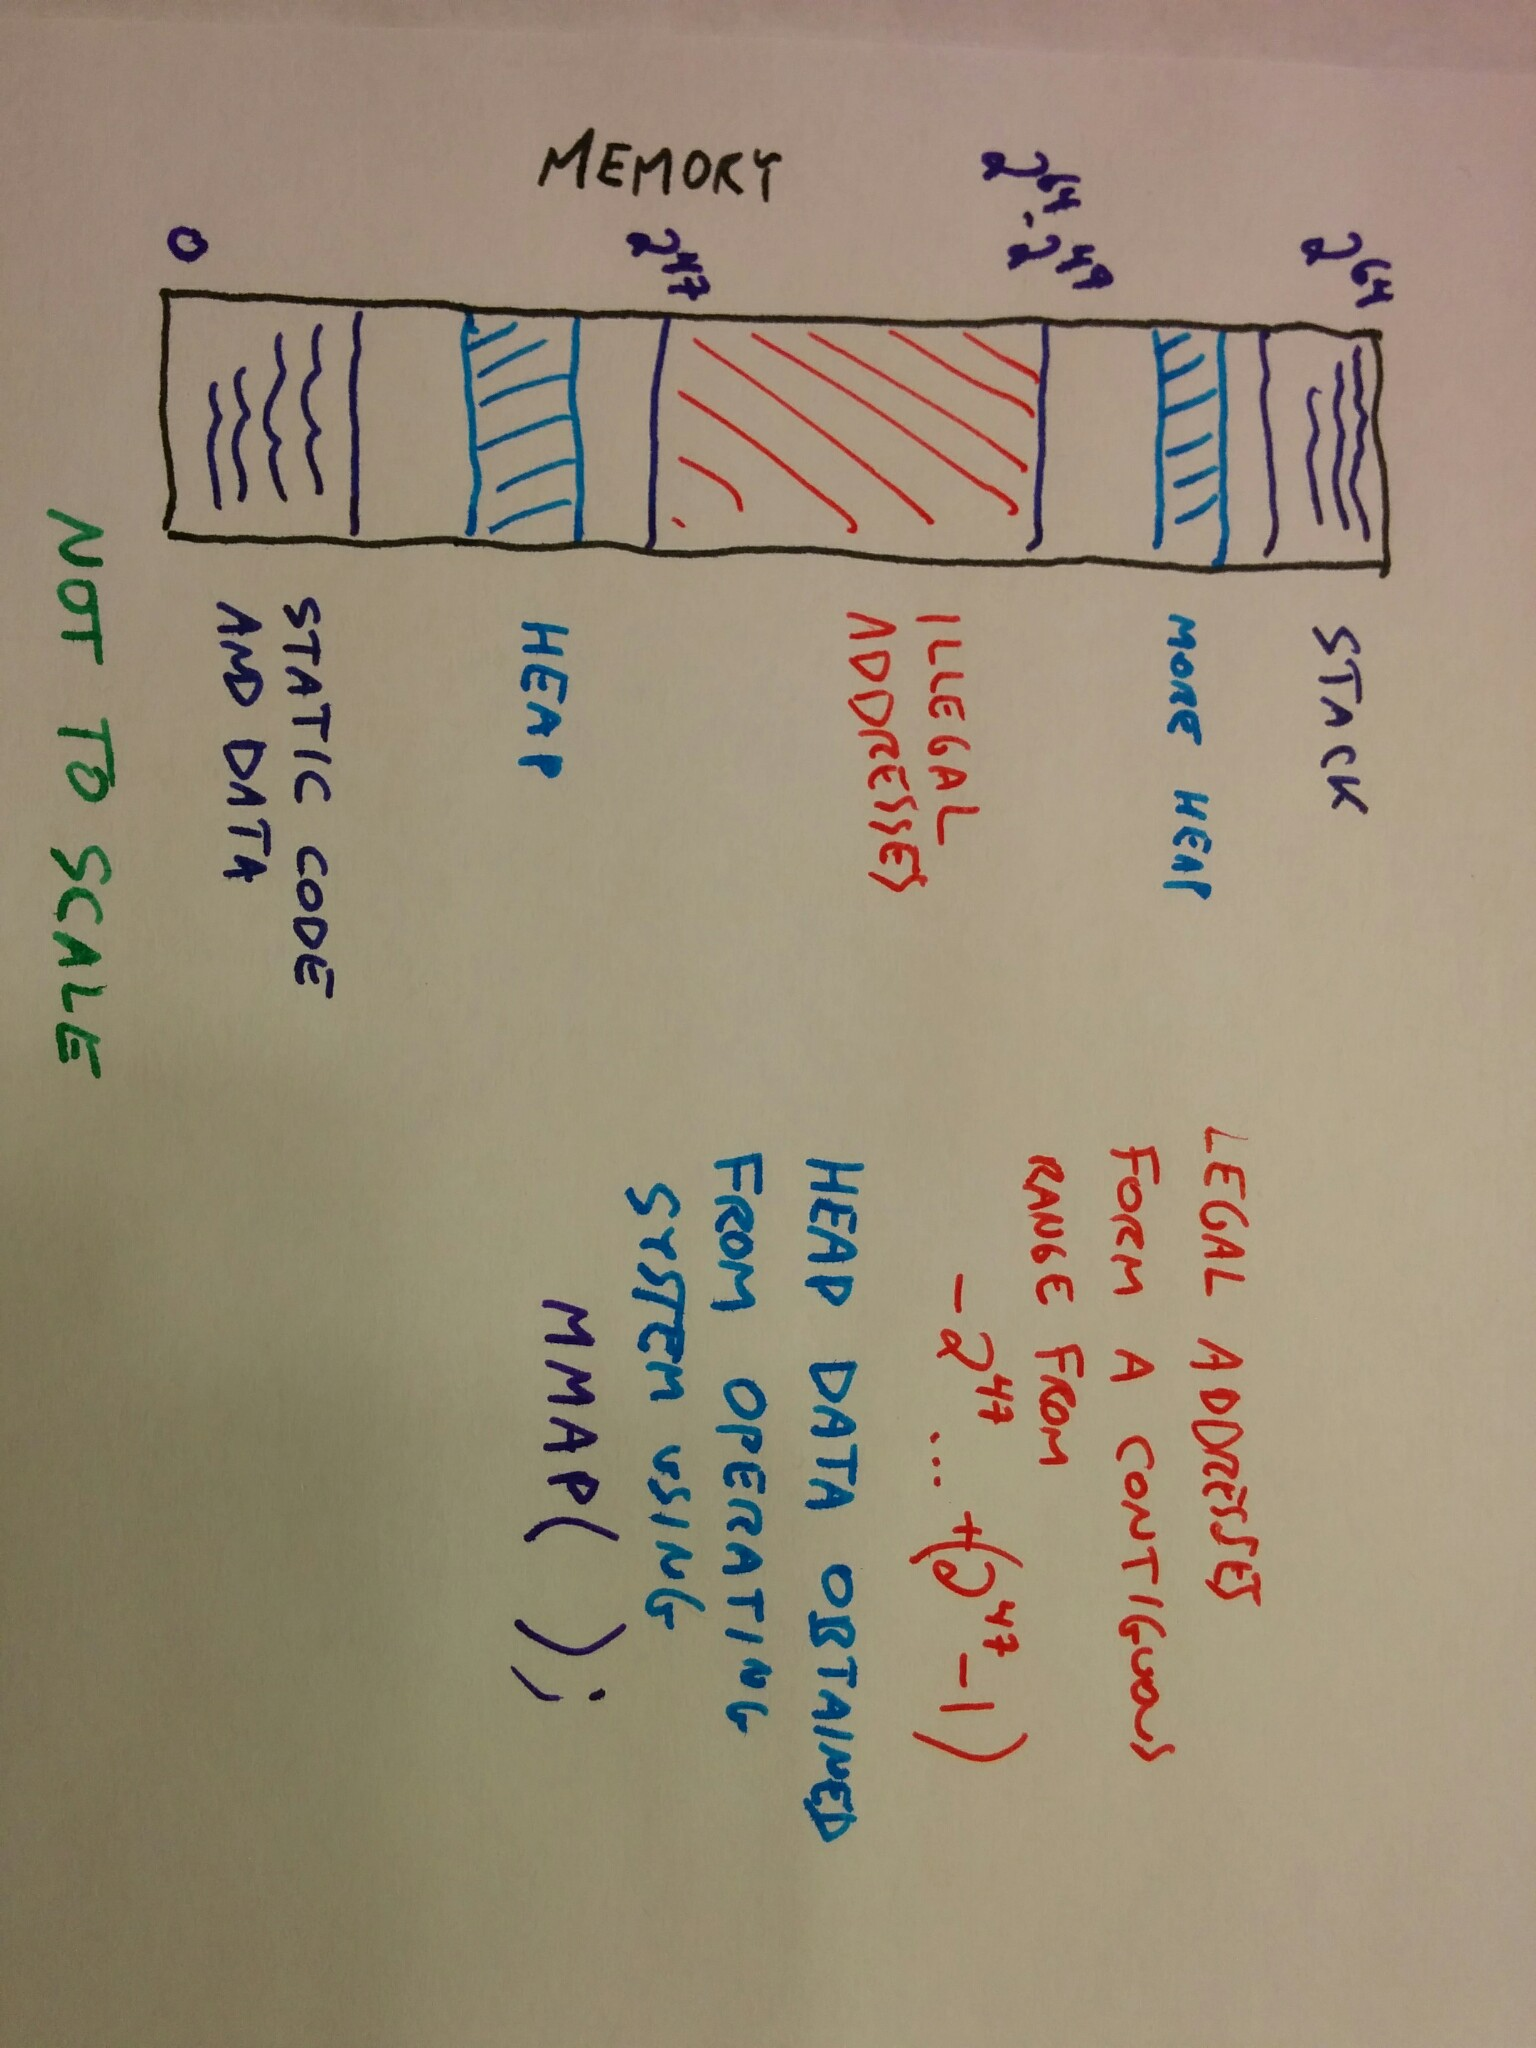
\includegraphics[width=3.35in,angle=90]{memory-layout.jpg}
\end{frame}

\begin{frame}
\frametitle{Boundary Tags [Knuth 73]}
\hspace*{-.35cm}
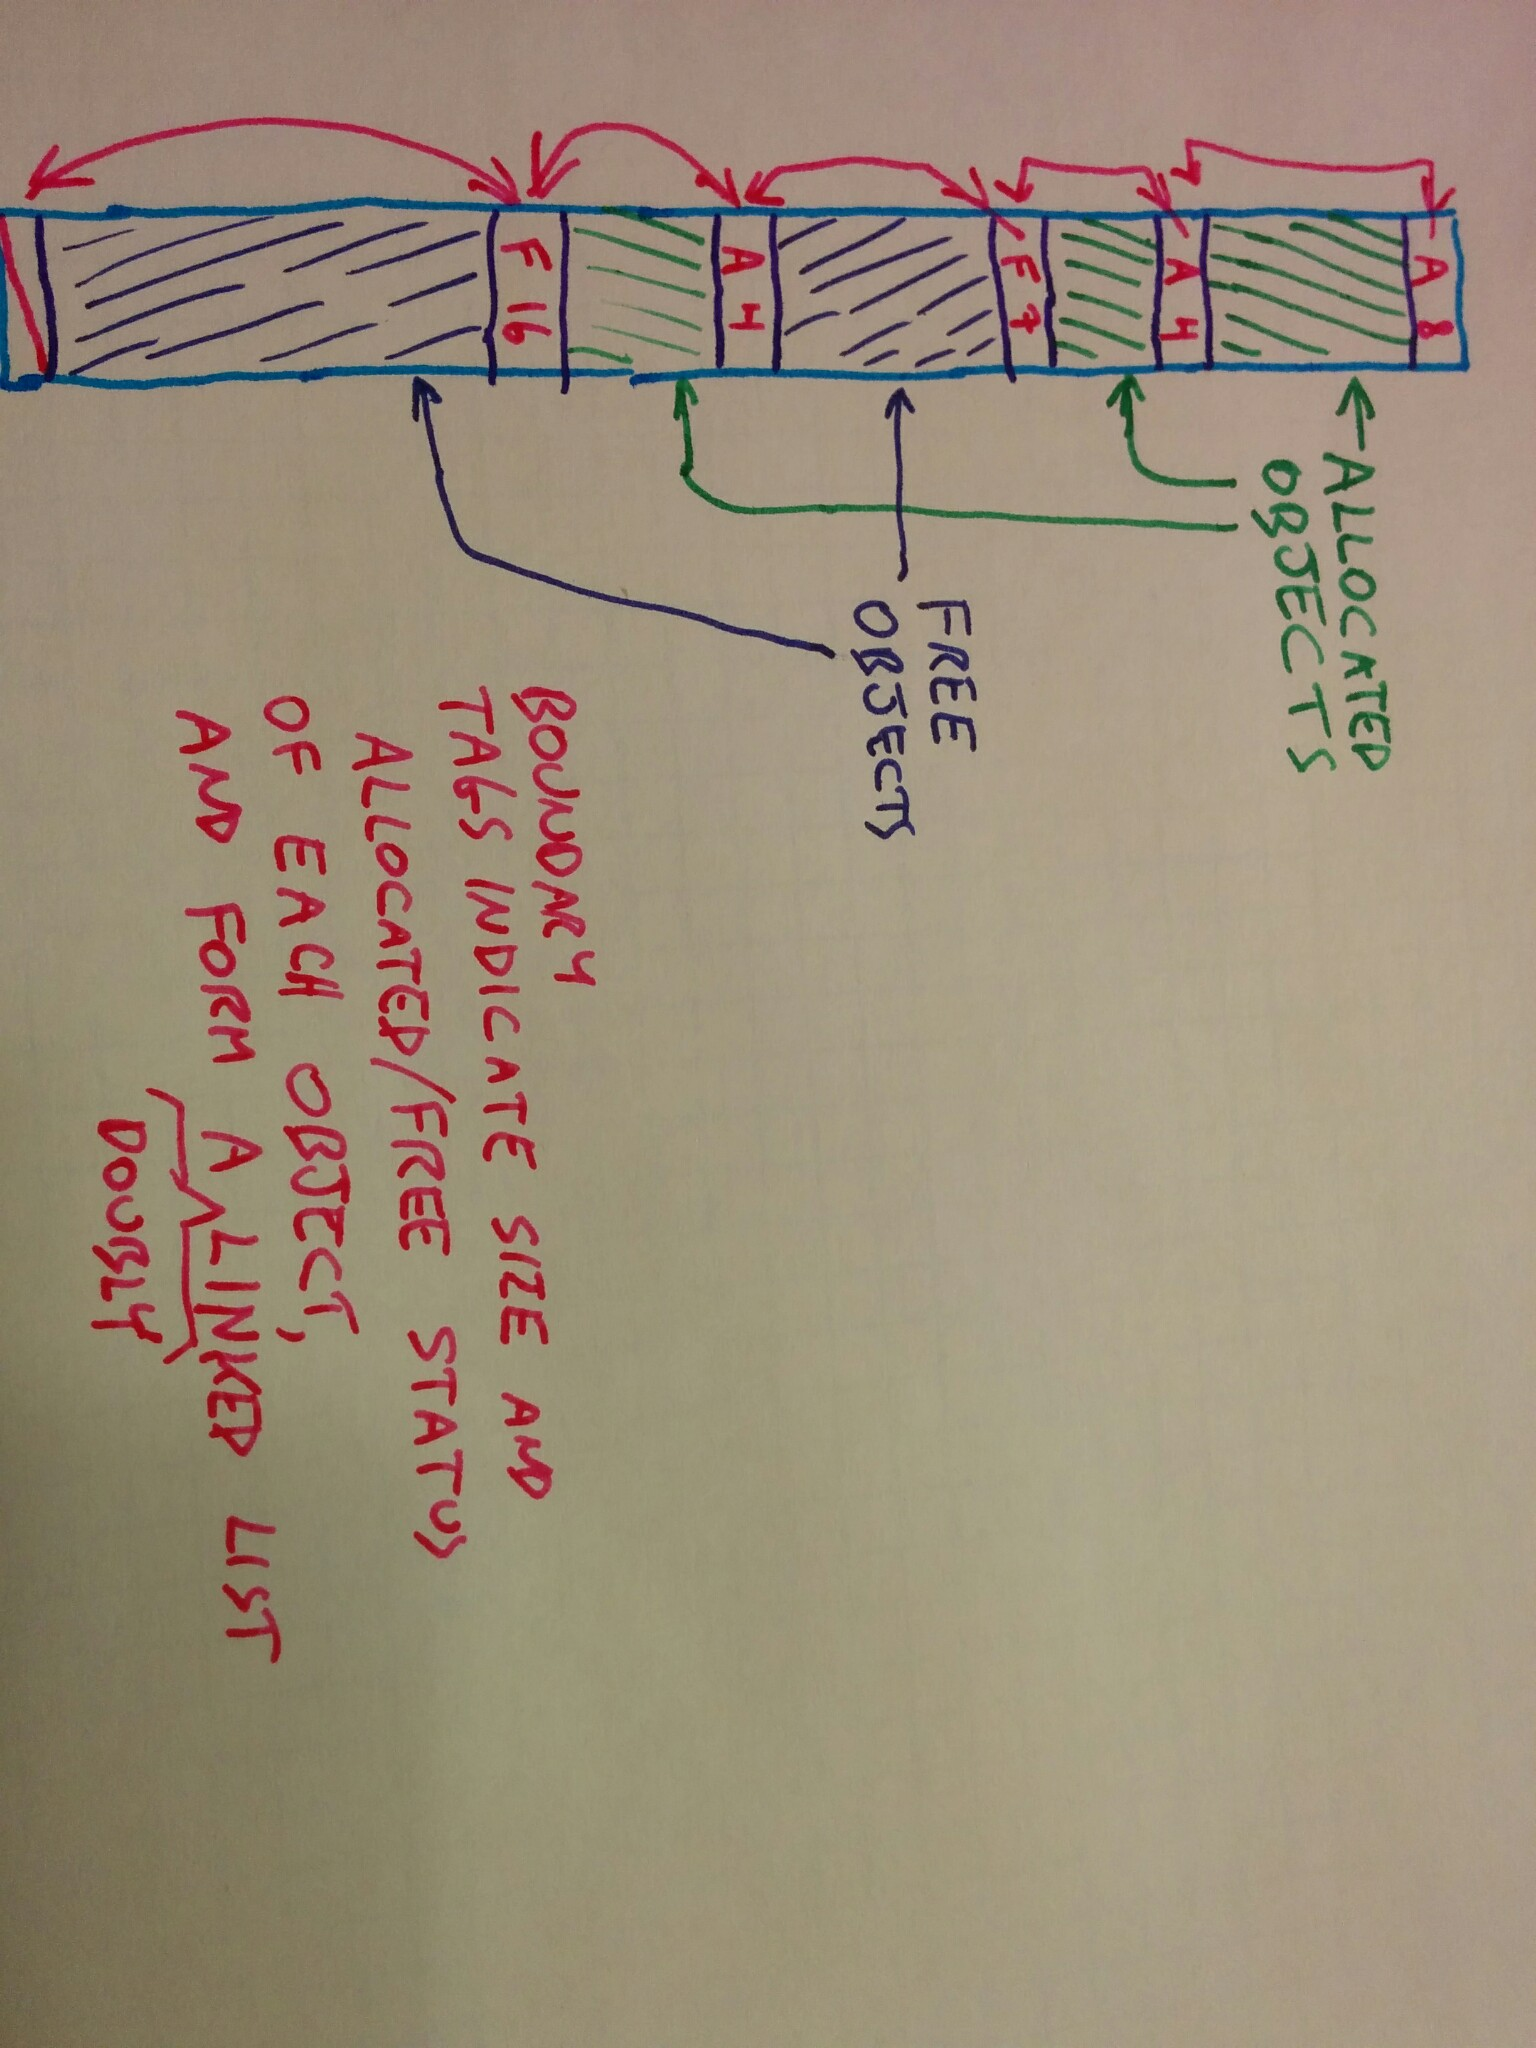
\includegraphics[width=3.35in,angle=90]{boundary-tag.jpg}
\end{frame}

\begin{frame}
\frametitle{Boundary Tags Are Simple and Slow}

\begin{itemize}
\item Allocating requires finding a suitable free region, possibly breaking
it in two.

\item Freeing requires merging adjacent free regions.

\item To run fast, the data structure gets more complex.

\item To run in a multithreaded environment, the DLmalloc protects its data
structures with a lock.

\item DLmalloc [Lea 87] uses boundary tags is slow, and for
  multithreaded code, it's even slower. 

\item  DLmalloc is the standard allocator in Linux and has changed little in 28 years.

\item Modern allocators use other data structures.
\end{itemize}
\end{frame}

\begin{frame}
\frametitle{Thread-local caches}

All modern allocators employ per-thread caches of recently freed objects.

\begin{itemize}
\item \mintinline{c}{free()} simply puts the object into the
  per-thread cache, and requires no locking.
\item \mintinline{c}{alloc()} requires no locking if the cache contains data.
\end{itemize}

What goes wrong?
\end{frame}

\begin{frame}[fragile]
\frametitle{Thread Caches Can Run Really Fast}

\begin{minted}{c}
// Thread A
while (1) free(malloc(16));

// Thread B
while (1) free(malloc(16));
\end{minted}
\end{frame}

\begin{frame}[fragile]
\frametitle{The Problem with Thread Caches}

The \texttt{malloc-test} workload [LeverBo00].

\begin{minted}{c}
queue Q;

// Thread A
while (1) Q.push(malloc(16));

// Thread B
while (1) free(Q.pop());
\end{minted}


If Thread~A allocates an object, and hands it to Thread~B which frees
the object, then Thread~B's cache fills up.

Allocators such as TBBmalloc [KukanovVo07] suffer unbounded space
blowups for this kind of workload, which seems to be the toughest workload.
\end{frame}

\begin{frame}
\frametitle{Useful Allocators Limit Space}

\begin{itemize}
\item Hoard [BergerMcBl00] provides a competitive space bound by careful
bookkeeping on the sizes of the thread cache.

\item JEmalloc [Evans06] provides similar bounds in practice by simply
limiting the size of the thread cache.

\item These days, JEmalloc seems much more popular than Hoard.

\item There are many other allocators [PTmalloc, TCCmalloc, LocklessMalloc, ...]

\item I wrote SuperMalloc.
\end{itemize}

\end{frame}

\begin{frame}
\frametitle{SuperMalloc is $>3\times$ faster}

{\small
% GNUPLOT: LaTeX picture with Postscript
\begingroup
  \fontfamily{ptm}%
  \selectfont
  \makeatletter
  \providecommand\color[2][]{%
    \GenericError{(gnuplot) \space\space\space\@spaces}{%
      Package color not loaded in conjunction with
      terminal option `colourtext'%
    }{See the gnuplot documentation for explanation.%
    }{Either use 'blacktext' in gnuplot or load the package
      color.sty in LaTeX.}%
    \renewcommand\color[2][]{}%
  }%
  \providecommand\includegraphics[2][]{%
    \GenericError{(gnuplot) \space\space\space\@spaces}{%
      Package graphicx or graphics not loaded%
    }{See the gnuplot documentation for explanation.%
    }{The gnuplot epslatex terminal needs graphicx.sty or graphics.sty.}%
    \renewcommand\includegraphics[2][]{}%
  }%
  \providecommand\rotatebox[2]{#2}%
  \@ifundefined{ifGPcolor}{%
    \newif\ifGPcolor
    \GPcolortrue
  }{}%
  \@ifundefined{ifGPblacktext}{%
    \newif\ifGPblacktext
    \GPblacktextfalse
  }{}%
  % define a \g@addto@macro without @ in the name:
  \let\gplgaddtomacro\g@addto@macro
  % define empty templates for all commands taking text:
  \gdef\gplbacktext{}%
  \gdef\gplfronttext{}%
  \makeatother
  \ifGPblacktext
    % no textcolor at all
    \def\colorrgb#1{}%
    \def\colorgray#1{}%
  \else
    % gray or color?
    \ifGPcolor
      \def\colorrgb#1{\color[rgb]{#1}}%
      \def\colorgray#1{\color[gray]{#1}}%
      \expandafter\def\csname LTw\endcsname{\color{white}}%
      \expandafter\def\csname LTb\endcsname{\color{black}}%
      \expandafter\def\csname LTa\endcsname{\color{black}}%
      \expandafter\def\csname LT0\endcsname{\color[rgb]{1,0,0}}%
      \expandafter\def\csname LT1\endcsname{\color[rgb]{0,1,0}}%
      \expandafter\def\csname LT2\endcsname{\color[rgb]{0,0,1}}%
      \expandafter\def\csname LT3\endcsname{\color[rgb]{1,0,1}}%
      \expandafter\def\csname LT4\endcsname{\color[rgb]{0,1,1}}%
      \expandafter\def\csname LT5\endcsname{\color[rgb]{1,1,0}}%
      \expandafter\def\csname LT6\endcsname{\color[rgb]{0,0,0}}%
      \expandafter\def\csname LT7\endcsname{\color[rgb]{1,0.3,0}}%
      \expandafter\def\csname LT8\endcsname{\color[rgb]{0.5,0.5,0.5}}%
    \else
      % gray
      \def\colorrgb#1{\color{black}}%
      \def\colorgray#1{\color[gray]{#1}}%
      \expandafter\def\csname LTw\endcsname{\color{white}}%
      \expandafter\def\csname LTb\endcsname{\color{black}}%
      \expandafter\def\csname LTa\endcsname{\color{black}}%
      \expandafter\def\csname LT0\endcsname{\color{black}}%
      \expandafter\def\csname LT1\endcsname{\color{black}}%
      \expandafter\def\csname LT2\endcsname{\color{black}}%
      \expandafter\def\csname LT3\endcsname{\color{black}}%
      \expandafter\def\csname LT4\endcsname{\color{black}}%
      \expandafter\def\csname LT5\endcsname{\color{black}}%
      \expandafter\def\csname LT6\endcsname{\color{black}}%
      \expandafter\def\csname LT7\endcsname{\color{black}}%
      \expandafter\def\csname LT8\endcsname{\color{black}}%
    \fi
  \fi
  \setlength{\unitlength}{0.0500bp}%
  \begin{picture}(4320.00,2580.00)%
    \gplgaddtomacro\gplbacktext{%
      \csname LTb\endcsname%
      \put(538,558){\makebox(0,0)[r]{\strut{}\footnotesize 0}}%
      \csname LTb\endcsname%
      \put(538,1236){\makebox(0,0)[r]{\strut{}\footnotesize$50$M}}%
      \csname LTb\endcsname%
      \put(538,1914){\makebox(0,0)[r]{\strut{}\footnotesize$100$M}}%
      \csname LTb\endcsname%
      \put(538,2375){\makebox(0,0)[r]{\strut{}\footnotesize $134$M}}%
      \csname LTb\endcsname%
      \put(827,298){\makebox(0,0){\strut{} 1}}%
      \csname LTb\endcsname%
      \put(1615,298){\makebox(0,0){\strut{} 8}}%
      \csname LTb\endcsname%
      \put(2517,298){\makebox(0,0){\strut{} 16}}%
      \csname LTb\endcsname%
      \put(3418,298){\makebox(0,0){\strut{} 24}}%
      \csname LTb\endcsname%
      \put(4319,298){\makebox(0,0){\strut{} 32}}%
      \csname LTb\endcsname%
      \put(37,1466){\rotatebox{-270}{\makebox(0,0){\small \texttt{malloc()}'s per second}}}%
      \csname LTb\endcsname%
      \put(2516,19){\makebox(0,0){\small Producer threads}}%
      \put(2516,2282){\makebox(0,0){\strut{}}}%
      \csname LTb\endcsname%
      \put(2516,2281){\makebox(0,0){\strut{}}}%
      \colorrgb{0.00,0.39,0.00}%
      \put(2404,2185){\makebox(0,0)[r]{\strut{}\footnotesize SuperMalloc}}%
      \colorrgb{0.63,0.00,0.00}%
      \put(2742,639){\makebox(0,0)[r]{\strut{}\footnotesize dlmalloc}}%
      \colorrgb{0.63,0.00,0.63}%
      \put(4319,944){\makebox(0,0)[r]{\strut{}\footnotesize Hoard}}%
      \colorrgb{0.00,0.00,0.63}%
      \put(4094,1128){\makebox(0,0)[r]{\strut{}\footnotesize jemalloc}}%
    }%
    \gplgaddtomacro\gplfronttext{%
    }%
    \gplbacktext
    \put(0,0){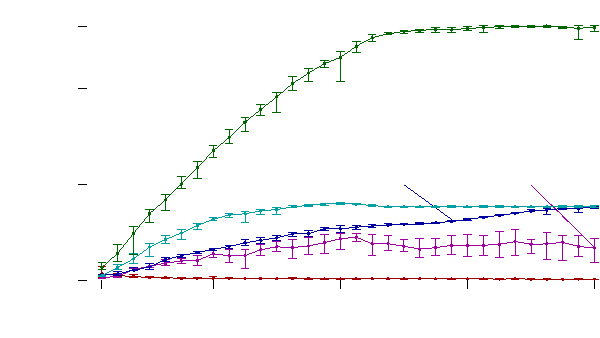
\includegraphics{new-malloc-test-1K-tempo-aggregated}}%
    \gplfronttext
  \end{picture}%
\endgroup

}

\texttt{malloc-test} on a 16-core, 32-hardware-thread, 2 socket,
2.4GHz E5-2665 Sandy Bridge.  Shown is the average of 8 trials, with
the error bars showing the max and min.

\end{frame}

\begin{frame}
\frametitle{Whence Came That Performance?}

\begin{itemize}
\item Per-CPU caching (the biggest performance advantage).
\item Simpler data structures (arrays instead of red-black trees).
\end{itemize}
\end{frame}

\begin{frame}
\frametitle{Costs of Locking vs. Cache Contention}

The cost of updating a variable in a multithreaded code is mostly in
cache contention, not locking.

\begin{center}
\begin{tabular}{rr}
  locked:                               contended global variable &    193.6ns \\
  locked: per cpu (and call \mintinline{c}{sched_getcpu()})  &     30.2ns \\
%  with lock:                    per cpu (cache getcpu, refresh/32) &     17.0ns \\
  no lock:                                              per thread &      3.1ns \\
  no lock:                                          local in stack &      3.1ns \\
\end{tabular}
\end{center}

\end{frame}

\begin{frame}
\frametitle{SuperMalloc Cache Strategy}

\begin{itemize}
\item A very small per-thread cache:  Only 10 items per size-bin needed to amortize the cost of the lock.
\item A small per-CPU cache: Only about 1 megabyte of objects per size-bin, since if the objects don't fit in the CPU cache the application will suffer cache misses anyway.
\item A medium global cache: A cache that is $O(P)$ bigger than a per-CPU cache.
\item The global data structures.
\end{itemize}
\end{frame}

\begin{frame}
\frametitle{Other Space and Time Savers}

\begin{itemize}
\item 2-mebibyte chunks of uniform-sized objects.
\item Arrays, not red-black trees, for chunk info.
\item Bitmaps for free list within a chunk.
\item Alloc-on-fullest-page heuristic.
\item \mintinline{c}{madvise(DONT_NEED)} to decommit memory.
\item Objects are a prime number of cache lines to reduce associativity conflicts.
\item Perform division (by those prime numbers) by multiplication-and-shift.
\item Use hardware transactional memory.
\item Prefetch cache lines before critical sections.
\end{itemize}
\end{frame}

\begin{frame}
\frametitle{Wishlist}

\begin{description}
\item[Cheap Uncommit:] I want \mintinline{c}{MADV_FREE}, which makes it cheap to give memory to the OS\@.  BSD has it.
 Better: the kernel should deliver a memory-pressure event.
\item[Lock-Aware Scheduling:] I want \mintinline{c}{schedctl()}, which advises the kernel to defer
  involuntary preemption briefly, reducing lock-holder preemption.  Solaris has it.
\item[Preload help:] Coding to preload cache is difficult.
\item[Late lock subscription:] Coding safely is difficult.
\item[Subscribable mutexes:] OS support to wait until a mutex is unlocked.
\end{description}
\end{frame}

\end{document}

\setlength{\unitlength}{0.01in}
\begin{picture}(200,335)
\put(10,100){{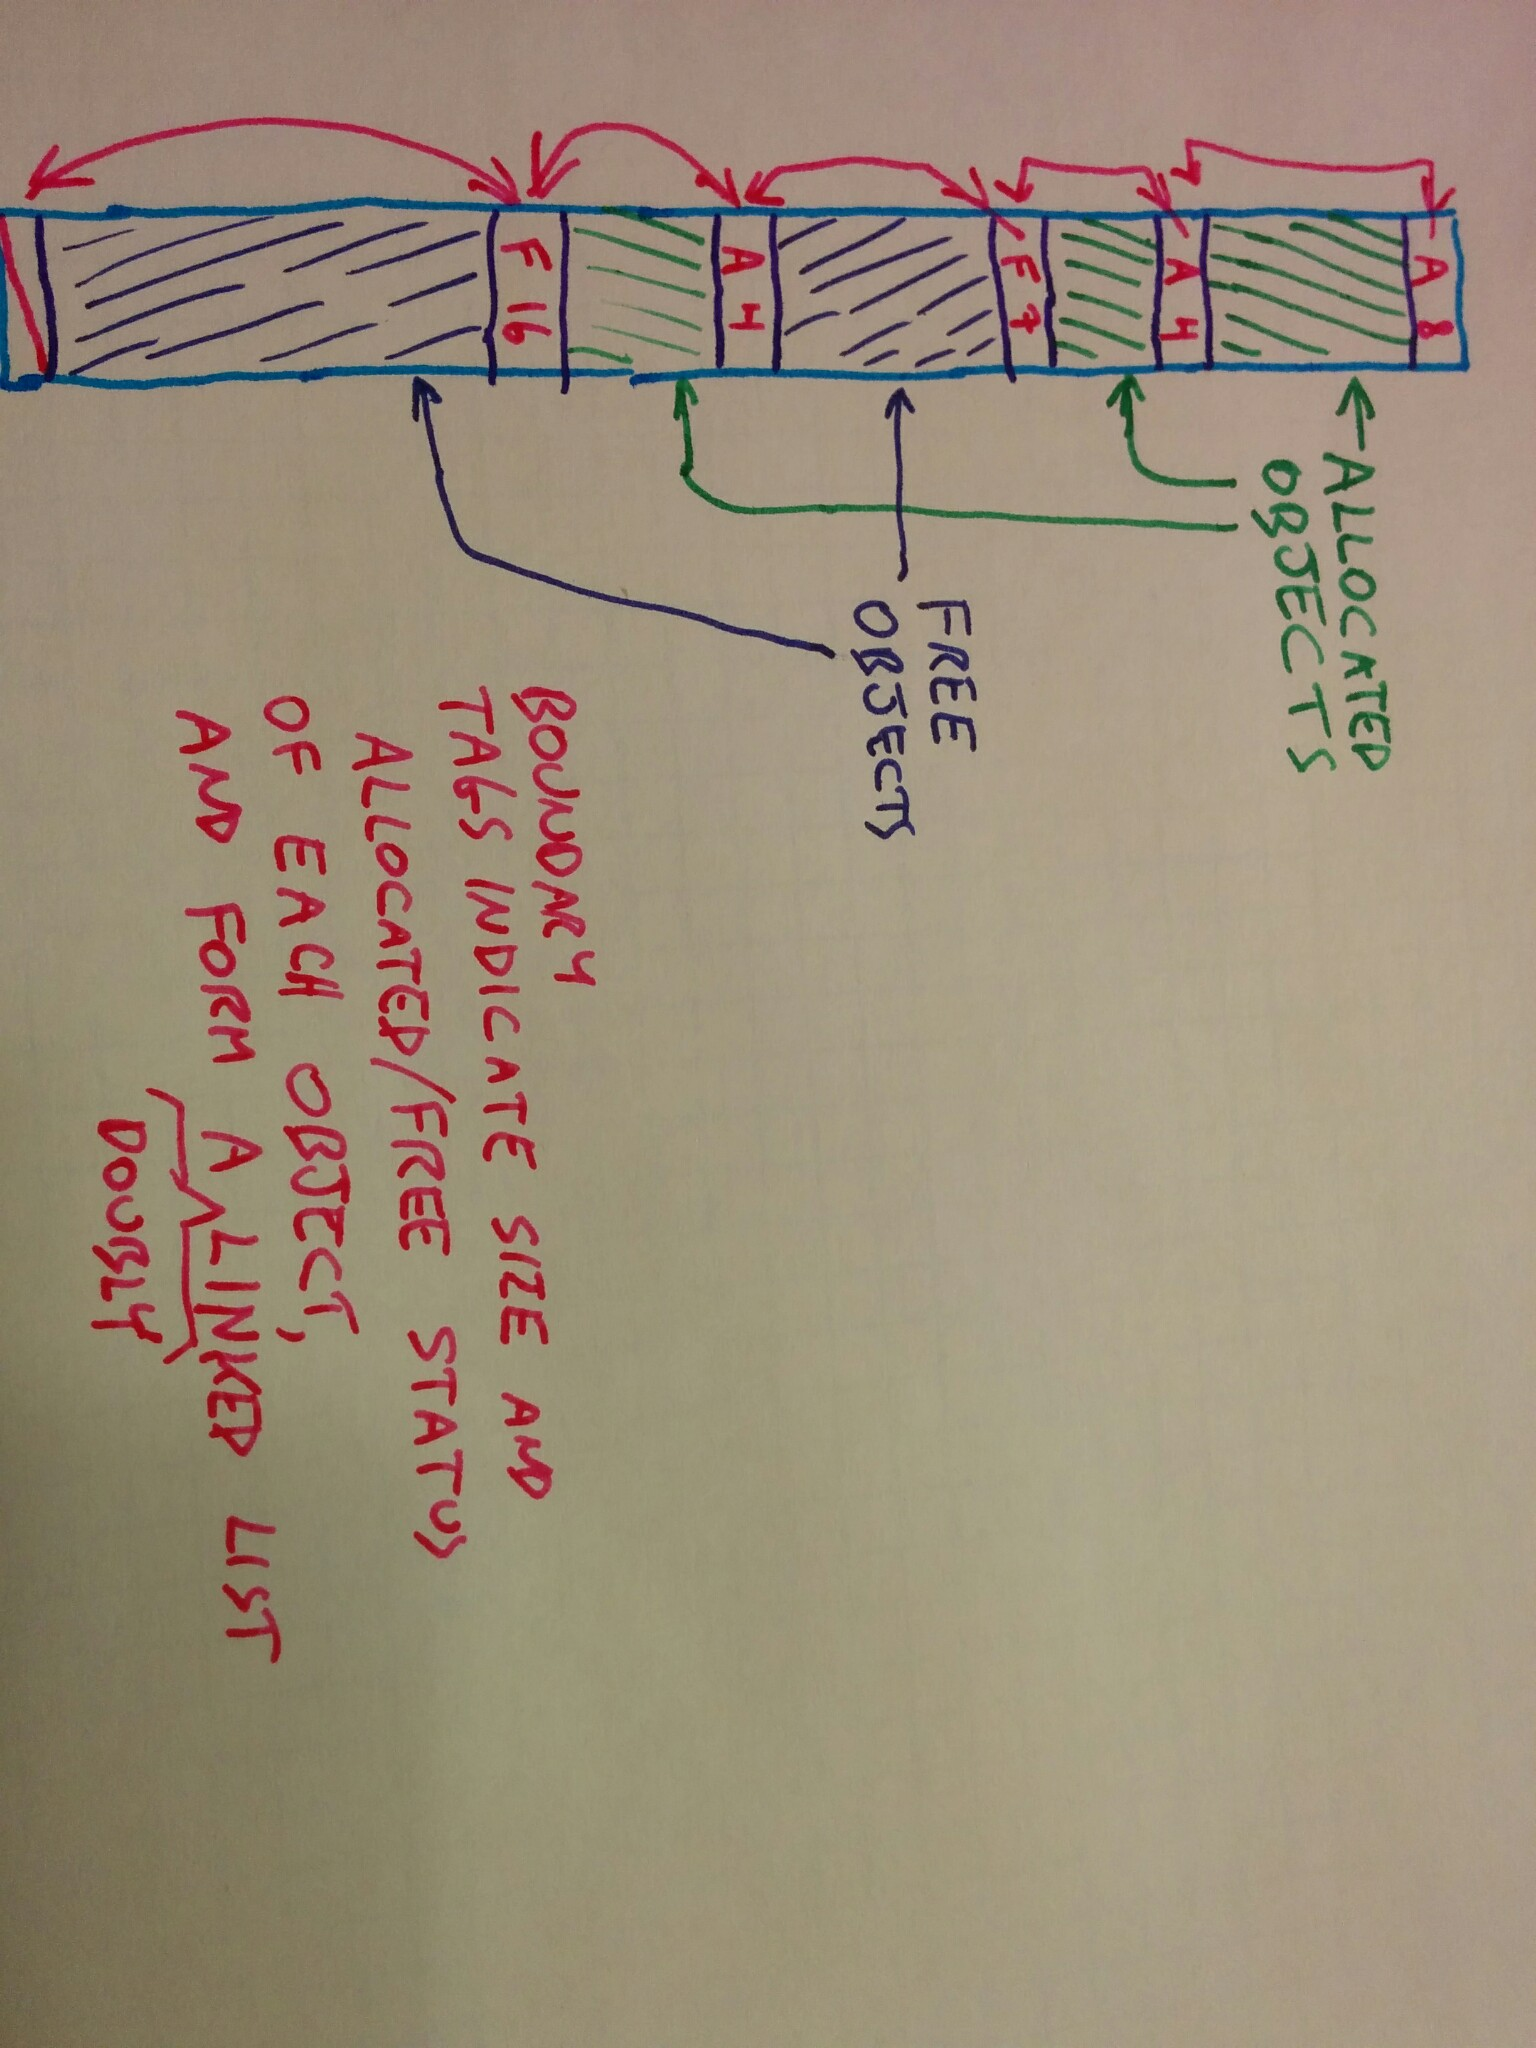
\includegraphics[width=3.35in,angle=90]{boundary-tag.jpg}
\end{picture}


malloc api

libc malloc uses boundary tags and a monolithic lock

scales badly with threads

tcmalloc uses per-thread cache (tc = thread cache)

tcmalloc works really well when a thread mallocs and frees as fast as it can.

tcmalloc works very badly when a thread mallocs, hands the object to another thread that frees.

hoard has a provably good scheme for managing these thread caches.

still a big performance hit on the table.  Show the graph that we can run faster on.

what does per-thread cache buy?  The issue is the cache contention not the lock

performance of locks and atomic operations for different 

implemenation:  small per-thread cache; per-cpu cache; global cache

other: Use a big array instead of a red-black tree

other: OS wish list.





